\documentclass[../main]{subfiles}

\begin{document}

\chapter{The Scratch execution model}\label{ch:scratch-execution-model}

\dictum[J. Maloney, M. Resnick, et al. \\ \textit{The Scratch Programming Language and Environment}]{Concurrency is often considered an advanced programming technique. Yet our everyday world is highly concurrent, so Scratch users
are not surprised that a sprite can do several things at once.}

The current Scratch execution model makes some choices which make it difficult to implement certain features of debuggers.
\marginnote{We encountered those difficulties in our work on Blink (\cref{ch:blink}).}
The root cause is the almost-cooperative threading model implemented by the current execution model.

These prevent us from allowing the debugger to behave as we would want: either the debugger would be less usable, or it would deviate from how Scratch executes in normal mode.
Both are not desirable.
Since these issues are also present during normal execution of Scratch code, although in practice infrequently, we decided the execution model itself should be modified.

We begin this chapter with an in-depth exploration of how the current execution model of Scratch works and behaves.
This is necessary for a good understanding of the next section, where we discuss what the issues with it are.

Next, we detail what a solution would look like and propose a family of modified execution models.
We then evaluate these models with a set of metrics to illustrate how their modifications affect Scratch's behaviour in real-life projects.
Finally, we apply one of these models to the debugger to illustrate that we can now use the debugger without the execution deviating from the normal mode.

\begin{listing}
    \centering
    \begin{subfigure}{0.45\textwidth}
        \centering
        \begin{scratch}[scale=0.7]
            \blockinit{when \greenflag{} clicked}
            \blockmove{move  \ovalnum{100} steps}
            \blockmove{turn \turnleft{} \ovalnum{90} degrees}
            \blockmove{move  \ovalnum{100} steps}
            \blockmove{turn \turnleft{} \ovalnum{90} degrees}
            \blockmove{move  \ovalnum{100} steps}
            \blockmove{turn \turnleft{} \ovalnum{90} degrees}
            \blockmove{move  \ovalnum{100} steps}
            \blockmove{turn \turnleft{} \ovalnum{90} degrees}
        \end{scratch}
    \end{subfigure}
    \begin{subfigure}{0.45\textwidth}
        \centering
        \begin{scratch}[scale=0.7]
            \blockinit{when \greenflag{} clicked}
            \blockrepeat{repeat \ovalnum{4}}{
                \blockmove{move  \ovalnum{100} steps}
                \blockmove{turn \turnleft{} \ovalnum{90} degrees}
            }
        \end{scratch}
    \end{subfigure}
    \caption{Two Scratch programs that seeminlgy produce the same result: the sprite moves in a square of 100 steps, and finally stops at the same position as the start of the progam.}
    \label{lst:scratch-two-programs}
\end{listing}

\section{Elements of a Scratch program}\label{sec:elements-of-a-scratch-program}

A Scratch program consists of zero or more sprites and a stage (see also \cref{ch:scratch-the-programming-language}).
The stage is the background and is always present.
The other visual entities are the sprites: these are drawn on the stage.
Together, these are called targets.
For the most part, the stage can be considered as another sprite, albeit with a special function.
All sprites have their own local state: the variables and visual properties of the sprite (e.g.\ position, size, bounding box, colour, direction).
Due to its special role, the stage misses some of these properties (e.g.\ it does not have a size, direction, or position).
The variables of the stage are also global: all sprites can access and change this variable.

Code-wise, the Scratch blocks are organized into categories (see \cref{subsec:using-the-environment-and-the-blocks}).
However, in this case, it is useful to look at their technical type, which corresponds to their shape.
In total, there are seven types of blocks:

\begin{enumerate}[noitemsep]
    \item Hat blocks \scratchinline{\blockinit{\hspace{1em}\dots\hspace*{1em}}}, which are placed at the start of a script (they are named hat blocks since they visually sit on top of a script).
        A script can only have one hat block.
        They function as event listeners, which trigger execution of the script if the event occurs.
    \item Stack blocks \scratchinline{\blockmove{\hspace{1em}\dots\hspace*{0.5cm}}}, representing program statements.
        These are the most common blocks.
        They are called stack blocks since they are stacked on top of each other.
    \item C blocks \scratchinline{\blockif{\hspace{1em}\dots\hspace*{1em}}{\blockspace[0.2]}}, which are named after their shape.
        They are used for most of the control flow blocks: loops and branches.
        The variant for the if/else block is sometimes named an E block, since it has two slots.
    \item Reporter blocks \setscratch{baseline=c,scale=0.5}\ovalmove{\hspace{1em}\dots\hspace*{1em}}, act as variables or values and can be slotted into other blocks.
        Operators that result in a value also have this shape.
    \item Boolean blocks \setscratch{baseline=c,scale=0.5}\boolsensing{\hspace{1em}\dots\hspace*{1em}}, which are analogous to reporter blocks, but result in a boolean.
    \item Cap blocks \scratchinline{\blockstop{\hspace{1em}\dots\hspace*{1em}}}, which end a script: no blocks can be added afterwards.
        Note that the infinite loop block, for example, is both a C block and a cap block.
    \item Custom blocks \scratchinline{\initmoreblocks{define\hspace{1em}\dots\hspace*{1em}}}, which define ``procedures''.
\end{enumerate}

\section{Related work}\label{sec:execution-related-work}

There exists no full formal description of the Scratch execution model.
Instead, the execution model is defined informally, based on the implementation of the Scratch virtual machine.
In~\autocite{maloneyScratchProgrammingLanguage2010a}, the threading model is considered informally.
The largest amount of work is published in a series of papers by the \emph{Chair of Software Engineering II} group.

First, in~\autocite{stahlbauerTestingScratchPrograms2019}, the authors propose a formalization of three aspects: the user perspective, a syntactic model and a semantic model.
They propose that the semantics of Scratch can be described using a memory model based on message passing.
Then, in~\autocite{stahlbauerVerifiedScratchProgram2020} the authors develop LeILa, an intermediate language to which Scratch projects can be translated, with an intended use of performing analysis on Scratch projects.
The authors also provide formalizations of LeILa, but use approximations in some areas.
Also,~\autocite{gotzModelbasedTestingScratch2022} models the state-based behaviour of Scratch programs using a finite state machine.
Finally, in~\autocite{deinerAutomatedTestGeneration2023} the authors delve deeper into the actual execution of the virtual machine, while also proposing some modifications to it, for example, to make execution deterministic.

\section{The current execution model}\label{sec:the-current-execution-model}

\subsection{Execution of a Scratch program}\label{subsec:execution-of-a-scratch-program}

\marginnote{Arguably, it is more of a concrete syntax tree, as e.g. the position of blocks is also saved. However, in Scratch's case, the differences are minimal, so we call it an abstract syntax tree, as Scratch themselves do.}
When executing Scratch code, the virtual machine transforms the blocks into an abstract syntax tree.
These are organized by target, and every script of every target results in a thread inside the virtual machine.
These are green threads: implemented fully in the virtual machine.

The virtual machine is thus responsible for scheduling these threads.
A schematic overview of the interaction between the different parts is \cref{fig:blink-architecture}.
It uses an almost-cooperative threading model, which \citeauthor{maloneyScratchProgrammingLanguage2010a} call the ``Scratch threading model''~\autocite{maloneyScratchProgrammingLanguage2010a}.
This means it is mostly non-preemptive: the virtual machine will not interrupt threads at arbitrary points in their execution.
The threads must voluntarily yield control, or reach a limited set of points in their execution.
The rational is given in~\autocite{maloneyScratchProgrammingLanguage2010a}: ``Scratch builds concurrency control into its threading model in a way that avoids most race conditions, so that users do not need to think about these issues.
This is done by constraining where thread switches can occur.''.

At four well-defined points, a thread always yields, thus causing said thread switching:
\begin{enumerate}
    \item When a block is executed that has a fixed duration.
        There are a number of blocks that fall under this category.
        \scratchinline{\blockcontrol{wait \ovalnum{}}} is an obvious inclusion, but this also applies to \scratchinline{\blockmove{glide \ovalnum{} secs to x: \ovalnum{} y: \ovalnum{}}}, for example.
        \scratchinline{\blocksound{play sound \ovalsound*{} until done}} also falls under this category, even if there is no explicit time.
    \item When a block waits on execution of other blocks.
        For example, \scratchinline{\blockevent{broadcast \selectmenu{something} and wait}}.
    \item The last block of a loop (thus \scratchinline{\blockinfloop{forever}{\blockspace[0.2]}}, \scratchinline{\blockrepeat{repeat \ovalnum{}}{\blockspace[0.2]}}, and \scratchinline{\blockrepeat{repeat until \boolempty[1em]{}}{\blockspace[0.2]}}).
        This means thread switching will occur after every loop iteration.
    \item A recursive procedure call is detected.
        Scratch attempts to detect these (up to five levels of indirection) and will yield the thread on each call if it detects a recursive call.
\end{enumerate}

There is one exception: when using procedures ``without screen refresh'', Scratch will interrupt a thread that runs longer than \qty{500}{\milli\second}.
This is called the ``wrap timer'', and has some curious edge cases\footnote{\url{https://github.com/scratchfoundation/scratch-vm/issues/2834}}.

The threads are executed in a first-come, first-serve manner: there are no priorities nor changes in thread order.
The first thread is executed until it yields or ends, then the next thread, and so on.
We call the execution within one thread until it yields or ends a \term{turn}.
A thread can have one of three conceptual states: \emph{done}, \emph{running}, and \emph{yield}.

\begin{figure}
    \centering
    \includestandalone{scratch-model}
    \caption{Overview of the interplay between the threading model and the ``game loop''. Within one step (which is done 30 times per second), one or more ticks are executed. The arrow with \CircledText{2} illustrates this: after the first tick, another is started if less than \qty{75}{\percent} of the step time (the time one step has to complete, \qty{33}{\milli\second}) has been used, and a redraw has not been requested, and Scratch is not in turbo mode. Within one tick, a turn is executed for each thread \CircledText{1}: a thread executes until it terminates or the thread yields.}
    \label{fig:scratch-model-explained}
\end{figure}

\marginnote{Scratch 3 should actually run at 60 FPS; however Scratch enables a compatability mode by default, resulting in the 30 FPS.}
The virtual machine uses a \emph{fixed-time step with synchronization} main loop~\autocite{nystromGameProgrammingPatterns2014}, also called a \emph{synchronized coupled model}~\autocite{valenteRealTimeGame2005}.
This means that the virtual machine runs in \term{steps}: internally, the \texttt{step} function is called every \qty{33}{\milli\second} (so 30 times a second, commonly known as 30 frames per second).

In each step, the virtual machine will execute one or more ticks.
A \term{tick} is one turn in every thread: the first thread is executed until it yields or terminates, then the second thread and so on.
After the tick, a redraw is performed if needed (in practice this is always done, as the source code contains a to-do to implement selective redrawing).
After the first tick is finished, the virtual machine decides whether to run another tick (\cref{fig:scratch-model-explained}).
A new tick is started if less than \qty{75}{\percent} of the step time (the time one step has to complete, \qty{33}{\milli\second}) has been used and a redraw has not been requested.
Note that once a tick has started, it is run completely and cannot be stopped.
The arbitrary \qty{75}{\percent} is thus intended to prevent frame drops: steps that take longer than their allocated step time, meaning the next step is delayed.
Also, in practice, many blocks request a redraw, so in many Scratch projects, a step only ever runs one tick.

\begin{figure}
    \centering
    \begin{subfigure}{0.40\textwidth}
        \includestandalone{threading-no-loop}
    \end{subfigure}
    \begin{subfigure}{0.59\textwidth}
        \includestandalone{threading-with-loop}
    \end{subfigure}
    \caption{The execution of the two programs from \cref{lst:scratch-two-programs}. In the unrolled version (left), all code is executed in the first turn, meaning only one tick and step is needed. In the version with loop (right), the loop yields after each iteration, meaning the rest of the step is filled with idle time. In total, four steps are needed. }
    \label{fig:scratch-two-execution}
\end{figure}

A concrete example of the execution model is given by \cref{fig:scratch-two-execution}, which shows the execution of the programs of \cref{lst:scratch-two-programs}.
These programs have only one thread.
Since none of the blocks in the unrolled program yield the thread, the full program is executed in one step.
In the other version, with a loop, the thread yields after each iteration of the loop, meaning the program needs four steps.
This does result in an observable difference: in the unrolled program, the sprite does not move visually.
As a redraw only happens between steps, the sprite is back at its original position.
In the looped version, the sprite moves four times (albeit very fast), as there is a redraw between each step.

\subsection{Implementation details}\label{subsec:implementation-details}

How different parts of the virtual machine implement the execution model from \cref{subsec:execution-of-a-scratch-program} is shown in \cref{fig:blink-architecture}.
When the user interface loads a project, it also starts the virtual machine.
This means that the game loop is active (this is done in the class \texttt{Runtime}).

New threads are only created in two scenarios:
\begin{itemize}[noitemsep]
    \item Code needs to be executed, either because an event triggered some hat blocks (green flag, key press, etc.) or because the user clicked on some blocks.
    \item When ``stage monitors'' or watchers are active.
        These are used in the user interface to show the value of variables or properties.
        The watchers for variables also allow the user to change the value of the variable.
\end{itemize}

The \texttt{Runtime} calls the method \mintinline{javascript}{stepThreads} in the \texttt{Sequencer} class.
This class is responsible for implementing the ticks.
After each tick, done threads are removed, and a new tick is started if possible.
It is also here that the thread status is managed.
While there are three conceptual statuses, the implementation has five:
\begin{description}[noitemsep]
    \item[\texttt{done}] The thread has finished executing all blocks and will be removed after this tick.
    \item[\texttt{running}] The thread is being executed and has more blocks to execute.
        It will be scheduled again next tick.
    \item[\texttt{yield}] The thread is waiting an amount of time.
        The thread is scheduled again next tick to see if the wait time is over.
    \item[\texttt{promise wait}] The thread is waiting for a JavaScript promise to be resolved, after which the thread will be set to \texttt{running}.
    \item[\texttt{yield tick}] The thread yields until the next step.
        The purpose of this status seems to be some performance optimizations to aid with benchmarking\footnote{\url{https://github.com/scratchfoundation/scratch-vm/pull/1211}}.
\end{description}

Each thread maintains a stack structure.
The \texttt{Sequencer} will then look up the next block on said stack, and if there is one, it will call the \texttt{Execute} class.
That class will actually execute the block on the stack.
For normal blocks (confusingly called ``stack blocks'', since they stack in a script), the current block is popped from the stack, the block is executed, and the next block is put on the stack.
The stack is only useful when working with C-blocks or procedures.
For example, C blocks will push the first block in their slot on the stack.
In the case of a loop, a counter is saved in the stack frame to determine how many times the loop should be run.
The exact implementation of the stack is less relevant for this chapter, so it is left to the reader to browser the source code.

\section{Limitations of the execution model}\label{sec:limitations-of-the-execution-model-for-the-debugger}

This section illustrates a few limitations of the current execution model, first in general and then specifically for the debugger.

\subsection{In general}\label{subsec:in-general}

\begin{listing}
    \centering
    \begin{scratch}[scale=0.6]
        \blockinit{when \greenflag{} clicked}
        \blockmove{go to x: \ovalnum{0} y: \ovalnum{112}}
        \blockpen{erase all}
        \blockpen{set pen color to \pencolor{ppcolor}}
        \blockpen{set pen size to \ovalnum{5}}
        \blockpen{pen down}
        \blockmove{point in direction \ovalnum{108}}
        \blockrepeat{repeat \ovalnum{4}}{
            \blockmove{move \ovalnum{80} steps}
            \blockmove{turn \turnright{} \ovalnum{36} degrees}
            \blockmove{move \ovalnum{80} steps}
            \blockmove{turn \turnright{} \ovalnum{36} degrees}
        }
        \blockpen{pen up}
    \end{scratch}
    \hspace{3em}
    \begin{scratch}[scale=0.6]
        \blockinit{when \greenflag{} clicked}
        \blockinfloop{forever}{
            \blockif{if \boolsensing{touching color \pencolor{blue}} then}{
                \blockstop{stop \selectmenu{all}}
            }
        }
    \end{scratch}
    \caption{The implementation, with a bug in the first script (left) and a non-working second script (right).}
    \label{lst:star-model-implementation}
\end{listing}

\begin{figure}
    \begin{subfigure}{0.45\textwidth}
        
\includegraphics[width=\textwidth]{star-before}
        \caption{The stage before execution.}
        \label{fig:star-exercise-model-before}
    \end{subfigure}
    \hfill
    \begin{subfigure}{0.45\textwidth}
        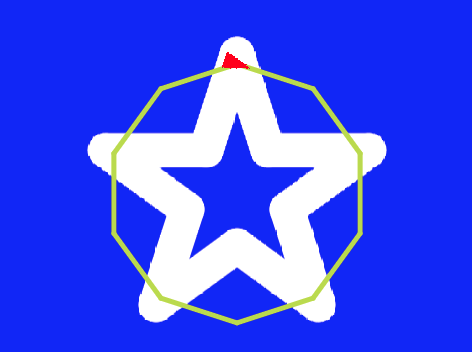
\includegraphics[width=\textwidth]{star-after}
        \caption{The stage after execution.}
        \label{fig:star-exercise-model-after}
    \end{subfigure}
    \caption{Result of running the implementation from \cref{lst:star-model-implementation} for the \emph{Star} exercise.}
    \label{fig:star-exercise-model}
\end{figure}

As \citeauthor{maloneyScratchProgrammingLanguage2010a} already mentioned, the Scratch threading model does not solve all issues with concurrency.
To illustrate this point, we will consider a variant on the \emph{Star} exercise from \cref{subsec:star-exercise}.
In this exercise, the goal is to let a sprite move around on a path without falling into the water (read touching a blue colour.)
\Cref{lst:star-model-implementation} shows an implementation for this exercise with an additional script that will stop execution if the sprite touches something blue.
We asked a number of educators that had experience with Scratch to predict the behaviour of this implementation.
All of them expected to execution to stop either when the sprite first touches the water or after the block when the sprite first touches the water.
However, as can be seen in \cref{fig:star-exercise-model-before,fig:star-exercise-model-after}, where the canvas is shown before and after running the code, the second script that should have stopped execution did not work.

The reason for this is the non-preemptive thread switching: the body of the loop is always executed atomically.
At the start of the loop, the sprite does not touch the water.
After execution of one iteration, the sprite is back on the path and does not touch the water.
Therefore, whenever the second script is executed, the sprite is not touching the water, which explains why the execution was not stopped.

Consider the original code in the \emph{Star} exercise from \cref{subsec:star-exercise}.
The second script there does not stop the execution, but uses Blink's pause block to halt the execution.
Using the current execution model, the pause block will not function for the same reasons mentioned above.

\subsection{Specifically for the debugger}\label{subsec:specifically-for-the-debugger}

One of the most basic features of any debugger is the ability to step through the code: executing one statement and then pausing the execution to allow the user to inspect the program state.
A debugger for Scratch also needs this functionality, and the debuggers that exist for Scratch all implement a stepping feature.

As described in \cref{sec:blink-software-architecture}, our debugger Blink takes a different approach to the stepping feature.
While most debuggers only execute one statement in a step, we believe it is useful to maintain the observed parallelism of Scratch in the debugger.
We thus aim to execute one step in every thread at the same time.
More concretely, we execute one block in every thread.
This approach allows users to keep focus on relevant threads without distractions from thread switches, which can be cumbersome in complex programs.
Users can thus focus on the script(s) they believe are involved in the failure while ignoring (correct) scripts running at the same time.

This approach does come at a price: it changes the execution model of Scratch.
Changing the execution model is not trivial due to two main considerations:

\begin{enumerate}
    \item If the execution model is only changed when debugging, the debugger does not debug the same program as when running the program.
        This can result in different behaviour, meaning the bugs for which the debugger is used are no longer present or new bugs, unique to the debugger, could be introduced.
    \item If the execution model is changed, we need to ensure that existing Scratch programs keep working and that we do not introduce concurrency problems, as the current execution model of Scratch was explicitly chosen to avoid those.
\end{enumerate}

We opt for the second option: modifying the Scratch execution model.
In the next section, we discuss what we changed, after which we investigate if existing Scratch projects can continue to work.

\section{New execution model}\label{sec:a-family-of-new-execution-models}

TODO: nieuwe model uitleggen

%When changing the execution model of Scratch, there is a multitude of parameters to change.
%For our debugger, the most important change is that we execute a single block at a time.
%A tick will thus execute a single block in each thread, before the thread yields.
%Since this has an impact on the execution speed (as more time is spent idling in each step), we need to intervene and change the ticks.
%There are multiple choices on how to do this, mainly variants of how many ticks are executed per step.
%The proposed new execution model will combine two strategies.
%In the normal mode, more ticks per step will be executed.
%
%\paragraph{More ticks per step}
%For example, we could decide to always execute two ticks per step.
%Since executing a single block per thread makes the execution time of a tick less variable, we could also execute as many ticks as possible in a step.
%This number would need to be determined and will be somewhat arbitrary.
%However, the existing limit of \qty{75}{\percent} is also somewhat arbitrary, so this need not be a problem.
%
%\paragraph{Run as fast as possible}
%Another approach is to remove the fixed-time step from Scratch: executing ticks as fast as possible.
%This can be achieved by running exactly one tick each step, and running the next step as soon as the previous one is ready.
%A consequence of this last change is that a Scratch program will run as fast as possible on the given hardware.
%Slower hardware and faster hardware will thus result in slower and faster executions respectively.
%This also potentially means that there will be a lot of redraws, of which some are useless as there were no visual changes.
%
%The built-in turbo mode in the current execution model is a combination of both: while the \qty{75}{\percent} is still honoured (thus a new tick will not be started if more than \qty{75}{\percent} of the step time is used), requests for redraws are ignored.
%Normally, a request for a redraw stops execution of new ticks, but in turbo mode, this is not the case.

\section{Evaluation of the new execution model}\label{sec:evaluation-of-the-new-execution-model}

\subsection{Evaluation of Scratch projects}\label{subsec:evaluation-of-scratch-projects}

Write about hwo most Scratch projects are not complex and do not use advanced techniques.


TODO

\section{Applying the new evaluation model on the debugger}\label{sec:applying-the-new-evaluation-model-on-the-debugger}

TODO

\section{Conclusion}\label{sec:conclusion}

TODO

\end{document}
